\begin{frame}{Gruppenstruktur}
    \begin{columns}
        \begin{column}{0.66\textwidth}
            
            \begin{algorithmblock}
                \begin{center}
                    $\mathcal{E}:y^2=x^3+486662x^2+x$
                \end{center}
               
        
            \end{algorithmblock}
            \begin{align*}
                \mathcal{E}(\mathbb{F}_{p^2})&=\{\mathcal{O}\}\cup \{(x,y)\in \mathbb{F}_{p^2}:y^2=x^3+Ax^2+x\}\\
                A&=\texttt{486662}\\
                p&=\texttt{2}^{\texttt{255}}-\texttt{19}\\
                \mathcal{E}^\prime(\mathbb{F}_{p^2})&=\{\mathcal{O}\}\cup (\mathcal{E}(\mathbb{F}_{p^2})\cap (\mathbb{F}_p\times\mathbb{F}_p))\\
                \#\mathcal{E}^\prime(\mathbb{F}_{p^2})&=\texttt{8}l\\
                l&=\#\langle P\rangle\\
                &=\texttt{2}^{\texttt{252}} +\texttt{0x14def9dea2f79cd65812631a5cf5d3ed}\\
                X(P)&=\texttt{9}\\
            \end{align*}
        \end{column}
        
        \begin{column}{0.5\textwidth}
            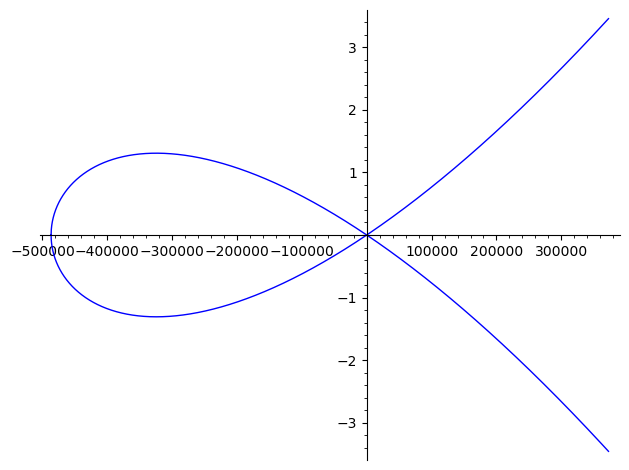
\includegraphics[width=\linewidth]{img/curve25519.png}
        \end{column}
    \end{columns}
    
\end{frame}
\begin{frame}{Gruppenstruktur}
    \begin{algorithmblock}
        \textbf{Gruppenoperationen.}\\
        Seien $P,Q\in \mathcal{E}(\mathbb{F}_{p^2})$:
         \end{algorithmblock}
        \begin{align*}
        \text{Neutrales Element}&: \; \mathcal{O}\,\text{(Punkt im Unendlichen)}\\
        \text{Punktaddition}&:P\oplus Q\\
        \text{Inverses Element}&: \ominus(x,y)=(x,-y) \\ &\quad P\oplus(\ominus P)=P\ominus P=\mathcal{O}\\
        \text{Skalarprodukt}&:[k]P=\underbrace{P\oplus\cdots\oplus P}_{k-Mal}
        \end{align*}
        
        
   
    
\end{frame}